\documentclass[14pt]{extbook}
\usepackage{multicol, enumerate, enumitem, hyperref, color, soul, setspace, parskip, fancyhdr} %General Packages
\usepackage{amssymb, amsthm, amsmath, bbm, latexsym, units, mathtools} %Math Packages
\everymath{\displaystyle} %All math in Display Style
% Packages with additional options
\usepackage[headsep=0.5cm,headheight=12pt, left=1 in,right= 1 in,top= 1 in,bottom= 1 in]{geometry}
\usepackage[usenames,dvipsnames]{xcolor}
\usepackage{dashrule}  % Package to use the command below to create lines between items
\newcommand{\litem}[1]{\item#1\hspace*{-1cm}\rule{\textwidth}{0.4pt}}
\pagestyle{fancy}
\lhead{Progress Quiz 3}
\chead{}
\rhead{Version C}
\lfoot{3148-2249}
\cfoot{}
\rfoot{Spring 2021}
\begin{document}

\begin{enumerate}
\litem{
Write the equation of the graph presented below in the form $f(x)=ax^2+bx+c$, assuming  $a=1$ or $a=-1$. Then, choose the intervals that $a, b,$ and $c$ belong to.
\begin{center}
    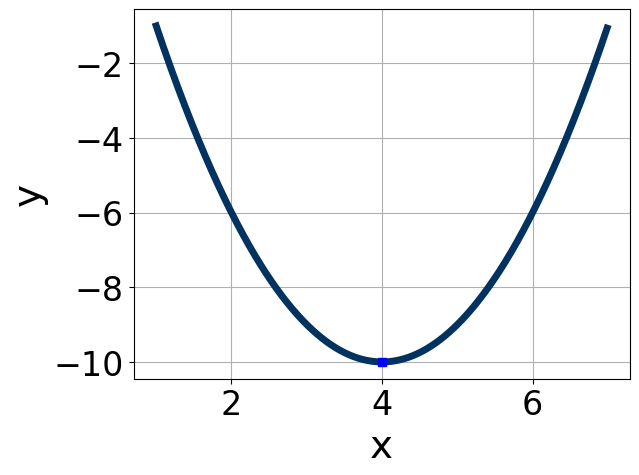
\includegraphics[width=0.5\textwidth]{../Figures/quadraticGraphToEquationCopyC.png}
\end{center}
\begin{enumerate}[label=\Alph*.]
\item \( a \in [-1.2, -0.3], \hspace*{5mm} b \in [-5, -3], \text{ and } \hspace*{5mm} c \in [-6, -4] \)
\item \( a \in [-1.2, -0.3], \hspace*{5mm} b \in [2, 5], \text{ and } \hspace*{5mm} c \in [-6, -4] \)
\item \( a \in [0.5, 2.1], \hspace*{5mm} b \in [2, 5], \text{ and } \hspace*{5mm} c \in [-1, 6] \)
\item \( a \in [-1.2, -0.3], \hspace*{5mm} b \in [2, 5], \text{ and } \hspace*{5mm} c \in [-4, -1] \)
\item \( a \in [0.5, 2.1], \hspace*{5mm} b \in [-5, -3], \text{ and } \hspace*{5mm} c \in [-1, 6] \)

\end{enumerate} }
\litem{
Factor the quadratic below. Then, choose the intervals that contain the constants in the form $(ax+b)(cx+d); b \leq d.$\[ 36x^{2} +60 x + 25 \]\begin{enumerate}[label=\Alph*.]
\item \( a \in [10.69, 13.51], \hspace*{5mm} b \in [-4, 9], \hspace*{5mm} c \in [2, 4.4], \text{ and } \hspace*{5mm} d \in [4, 9] \)
\item \( a \in [1.73, 2.18], \hspace*{5mm} b \in [-4, 9], \hspace*{5mm} c \in [13.8, 19.2], \text{ and } \hspace*{5mm} d \in [4, 9] \)
\item \( a \in [-0.37, 1.15], \hspace*{5mm} b \in [25, 33], \hspace*{5mm} c \in [0.1, 1.8], \text{ and } \hspace*{5mm} d \in [26, 32] \)
\item \( a \in [5.91, 7.49], \hspace*{5mm} b \in [-4, 9], \hspace*{5mm} c \in [5.9, 6.9], \text{ and } \hspace*{5mm} d \in [4, 9] \)
\item \( \text{None of the above.} \)

\end{enumerate} }
\litem{
Factor the quadratic below. Then, choose the intervals that contain the constants in the form $(ax+b)(cx+d); b \leq d.$\[ 36x^{2} +35 x + 6 \]\begin{enumerate}[label=\Alph*.]
\item \( a \in [1.7, 3.7], \hspace*{5mm} b \in [2, 4], \hspace*{5mm} c \in [11.24, 12.81], \text{ and } \hspace*{5mm} d \in [1, 5] \)
\item \( a \in [5.7, 11.7], \hspace*{5mm} b \in [2, 4], \hspace*{5mm} c \in [2.99, 5.07], \text{ and } \hspace*{5mm} d \in [1, 5] \)
\item \( a \in [-1.7, 1.5], \hspace*{5mm} b \in [7, 16], \hspace*{5mm} c \in [0.28, 1.69], \text{ and } \hspace*{5mm} d \in [27, 35] \)
\item \( a \in [12.4, 19.8], \hspace*{5mm} b \in [2, 4], \hspace*{5mm} c \in [1.81, 2.11], \text{ and } \hspace*{5mm} d \in [1, 5] \)
\item \( \text{None of the above.} \)

\end{enumerate} }
\litem{
Write the equation of the graph presented below in the form $f(x)=ax^2+bx+c$, assuming  $a=1$ or $a=-1$. Then, choose the intervals that $a, b,$ and $c$ belong to.
\begin{center}
    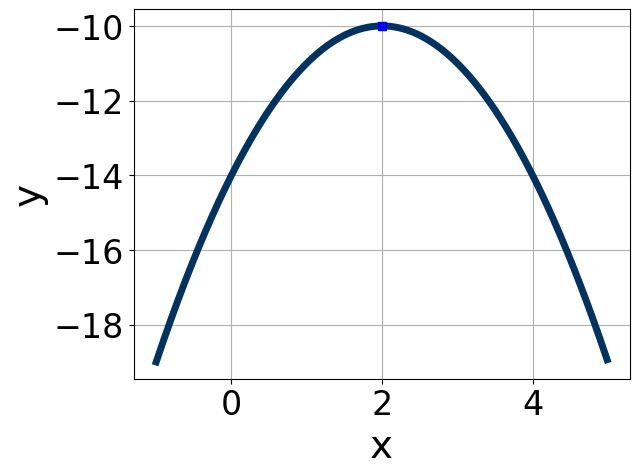
\includegraphics[width=0.5\textwidth]{../Figures/quadraticGraphToEquationC.png}
\end{center}
\begin{enumerate}[label=\Alph*.]
\item \( a \in [-0.4, 2.7], \hspace*{5mm} b \in [-8, -5], \text{ and } \hspace*{5mm} c \in [8, 9] \)
\item \( a \in [-0.4, 2.7], \hspace*{5mm} b \in [-8, -5], \text{ and } \hspace*{5mm} c \in [23, 29] \)
\item \( a \in [-2.5, -0.2], \hspace*{5mm} b \in [6, 12], \text{ and } \hspace*{5mm} c \in [-26, -21] \)
\item \( a \in [-0.4, 2.7], \hspace*{5mm} b \in [6, 12], \text{ and } \hspace*{5mm} c \in [8, 9] \)
\item \( a \in [-2.5, -0.2], \hspace*{5mm} b \in [-8, -5], \text{ and } \hspace*{5mm} c \in [-26, -21] \)

\end{enumerate} }
\litem{
Solve the quadratic equation below. Then, choose the intervals that the solutions $x_1$ and $x_2$ belong to, with $x_1 \leq x_2$.\[ 25x^{2} +15 x -54 = 0 \]\begin{enumerate}[label=\Alph*.]
\item \( x_1 \in [-45.07, -44.26] \text{ and } x_2 \in [29.85, 30.24] \)
\item \( x_1 \in [-5.68, -4.1] \text{ and } x_2 \in [0.28, 0.75] \)
\item \( x_1 \in [-9.76, -8.36] \text{ and } x_2 \in [-0.03, 0.27] \)
\item \( x_1 \in [-1.53, 0.93] \text{ and } x_2 \in [3.39, 4.24] \)
\item \( x_1 \in [-2.02, -1.74] \text{ and } x_2 \in [1.06, 1.45] \)

\end{enumerate} }
\litem{
Solve the quadratic equation below. Then, choose the intervals that the solutions belong to, with $x_1 \leq x_2$ (if they exist).\[ 20x^{2} -15 x -7 = 0 \]\begin{enumerate}[label=\Alph*.]
\item \( x_1 \in [-0.8, 0.9] \text{ and } x_2 \in [0.7, 2.5] \)
\item \( x_1 \in [-3.5, -0.7] \text{ and } x_2 \in [-0.2, 0.6] \)
\item \( x_1 \in [-7.3, -5.7] \text{ and } x_2 \in [20.6, 21.8] \)
\item \( x_1 \in [-28, -25.6] \text{ and } x_2 \in [27.4, 29.8] \)
\item \( \text{There are no Real solutions.} \)

\end{enumerate} }
\litem{
Solve the quadratic equation below. Then, choose the intervals that the solutions belong to, with $x_1 \leq x_2$ (if they exist).\[ -12x^{2} +14 x + 5 = 0 \]\begin{enumerate}[label=\Alph*.]
\item \( x_1 \in [-5.45, -0.45] \text{ and } x_2 \in [-1.6, 1.2] \)
\item \( x_1 \in [-19.44, -14.44] \text{ and } x_2 \in [2.5, 4.4] \)
\item \( x_1 \in [-22.3, -19.3] \text{ and } x_2 \in [21.2, 24] \)
\item \( x_1 \in [-1.29, 0.71] \text{ and } x_2 \in [0.9, 1.5] \)
\item \( \text{There are no Real solutions.} \)

\end{enumerate} }
\litem{
Graph the equation below.\[ f(x) = (x-3)^2 - 17 \]\begin{enumerate}[label=\Alph*.]
\begin{multicols}{2}\item 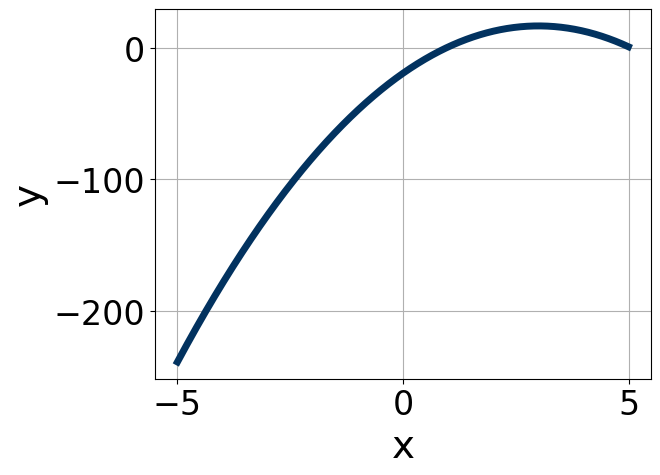
\includegraphics[width = 0.3\textwidth]{../Figures/quadraticEquationToGraphCopyAC.png}\item 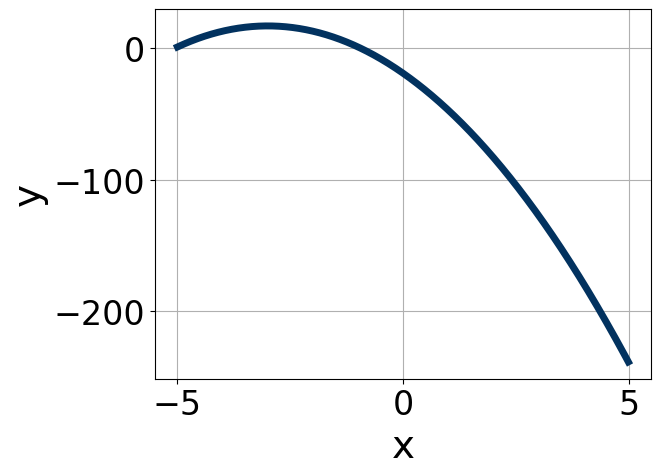
\includegraphics[width = 0.3\textwidth]{../Figures/quadraticEquationToGraphCopyBC.png}\item 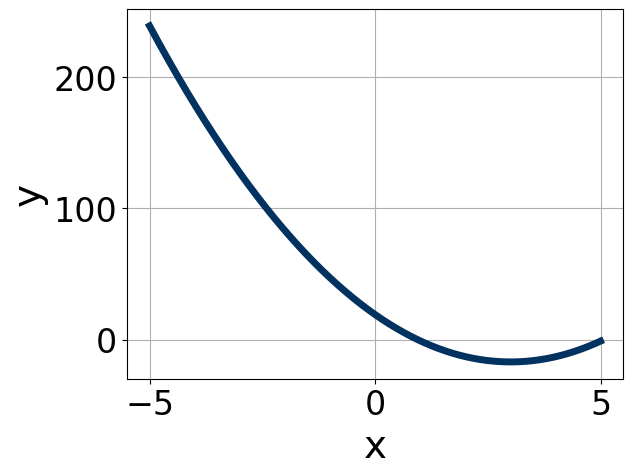
\includegraphics[width = 0.3\textwidth]{../Figures/quadraticEquationToGraphCopyCC.png}\item 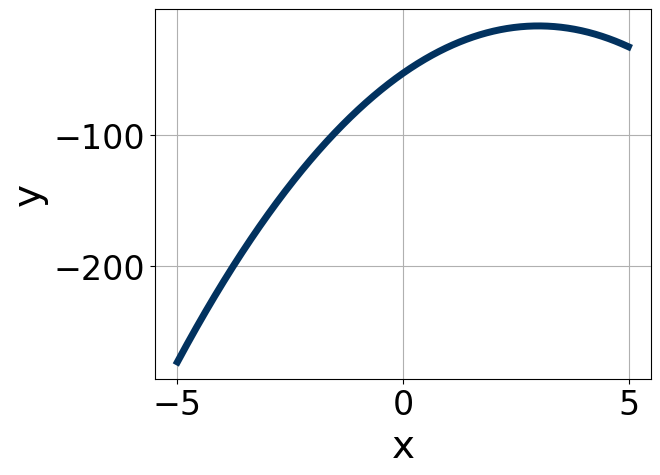
\includegraphics[width = 0.3\textwidth]{../Figures/quadraticEquationToGraphCopyDC.png}\end{multicols}\item None of the above.
\end{enumerate} }
\litem{
Graph the equation below.\[ f(x) = (x-2)^2 + 12 \]\begin{enumerate}[label=\Alph*.]
\begin{multicols}{2}\item 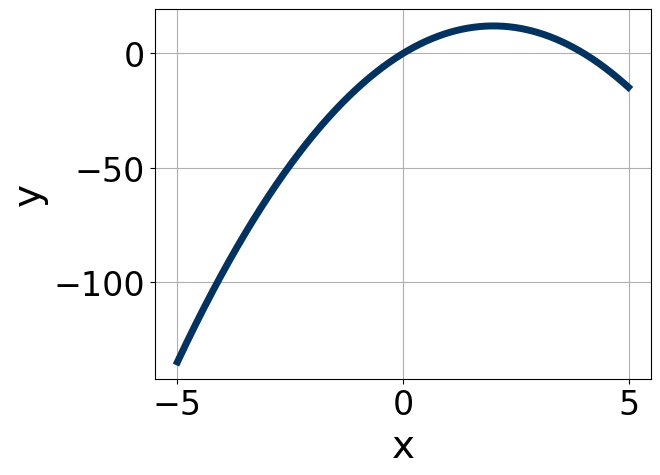
\includegraphics[width = 0.3\textwidth]{../Figures/quadraticEquationToGraphAC.png}\item 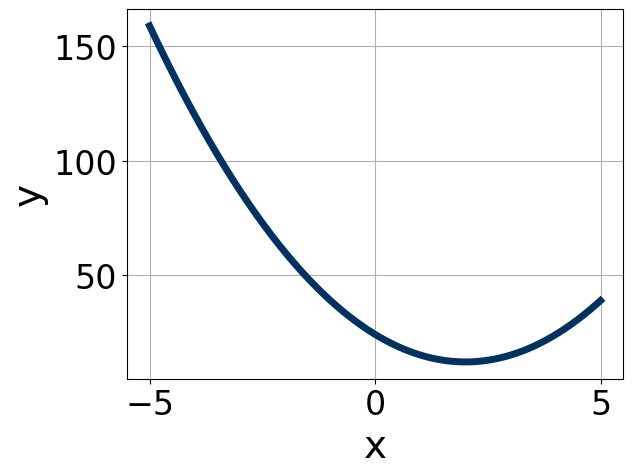
\includegraphics[width = 0.3\textwidth]{../Figures/quadraticEquationToGraphBC.png}\item 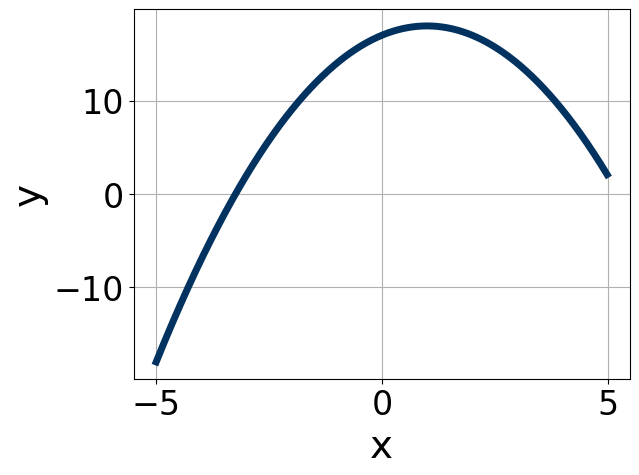
\includegraphics[width = 0.3\textwidth]{../Figures/quadraticEquationToGraphCC.png}\item 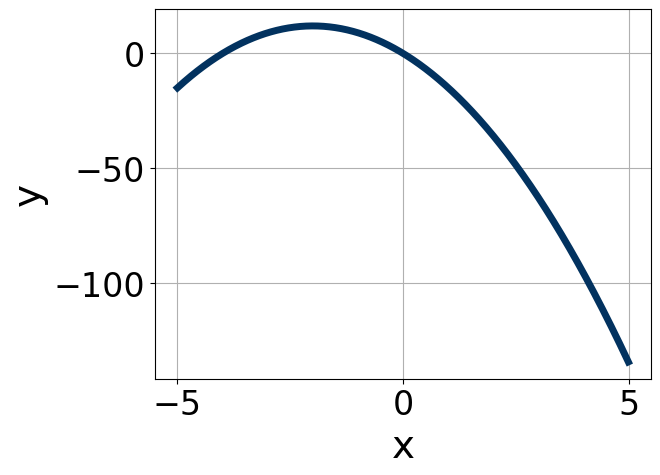
\includegraphics[width = 0.3\textwidth]{../Figures/quadraticEquationToGraphDC.png}\end{multicols}\item None of the above.
\end{enumerate} }
\litem{
Solve the quadratic equation below. Then, choose the intervals that the solutions $x_1$ and $x_2$ belong to, with $x_1 \leq x_2$.\[ 12x^{2} +11 x -36 = 0 \]\begin{enumerate}[label=\Alph*.]
\item \( x_1 \in [-1.72, -0.18] \text{ and } x_2 \in [3.69, 4.95] \)
\item \( x_1 \in [-3.63, -1.98] \text{ and } x_2 \in [1.06, 1.34] \)
\item \( x_1 \in [-4.71, -3.66] \text{ and } x_2 \in [0.58, 0.67] \)
\item \( x_1 \in [-28.26, -26.6] \text{ and } x_2 \in [15.84, 17.04] \)
\item \( x_1 \in [-10.26, -8.2] \text{ and } x_2 \in [-0.18, 0.65] \)

\end{enumerate} }
\end{enumerate}

\end{document}